\section{Introduction}
Aeroelastic models such as the Blade Element Momentum (BEM) models \cite{HandBook} play a critical role in the design, development, and optimization of modern wind turbines. A large number of BEM models have been developed to predict turbine responses such as structural loads and power output \cite{Vorpahl2013}. 

As a consequence of the relatively strong model assumptions at the basis of BEM theory, the results from BEM codes can be subject to significant uncertainties. For example, the effect of sheared inflow \cite{Madsen2012} is not naturally accounted for in the theory and needs to be incorporated via correction terms. Other major model uncertainties in BEM models are the time constant in dynamic stall models, the wake correction factor, the tip loss model parameter, and the lift- and drag-polars used to compute local aerodynamic forces. Especially for increasing turbine sizes, these model parameters are likely not sufficiently accurate \cite{Sayed2019}. 
%In other words, the uncertainty associated with the output of currently employed BEM models is rather large. 
% to arrive at robust BEM models that include an uncertainty estimate associated 

Recently, several papers have addressed the uncertainty in BEM model output by performing uncertainty propagation and sensitivity studies, e.g.\ \cite{Echeverria2017,Matthaus2017,Murcia2018,Robertson2018,Bos2019c}. In these studies, the focus in mainly on uncertainties in the external conditions (wind parameters) and/or uncertainty in the turbine specification (geometric parameters). Apart from understanding how uncertainty in the output is related to the different uncertain inputs, such sensitivity studies are very useful to reduce the number of parameters as needed for example in design optimization \cite{Echeverria2017}. However, the uncertainty in BEM model output as caused by uncertainty in the model formulation itself, e.g.\ through the values chosen for model parameters, has been given little attention. % (exceptions being the effect of aerodynamic properties studied in \cite{Bortolotti2019,Matthaus2017})\todo{this is also what we do}.

The goal of this work is to perform a systematic assessment of the uncertainty in model parameters in BEM models. We approach this by performing a global sensitivity analysis based on the Sobol expansion approach, which decomposes the total variance of the quantity of interest (model output) into contributions from individual parameters and their combinations, similar to \cite{Echeverria2017,Murcia2018, Rinker2016a}. We will employ the uncertainty quantification toolbox \texttt{UQLab} \cite{uqlab}, which computes the Sobol indices based on a sparse polynomial chaos expansion. The main novelty of the work lies in creating a generic framework that enables an advanced (global) sensitivity analysis of a relatively high number of uncertain parameters (e.g.\ 10-20), including both model and geometric uncertainties. The two key ingredients for this are efficient parameterization and the adaptive sparse polynomial expansion. This framework for sensitivity analysis is part of the so-called \textit{WindTrue} project, in which the long-term goal is the development of calibrated BEM models. Anticipating on this goal, we are using the NM80 wind turbine model from the Tjaereborg wind farm, for which extensive measurement data is available through the DanAero project \cite{Troldborg2013} and IEA Task 29  Phase IV (Phase IV is a follow-up of Task 29 Phase III \cite{Boorsma2018} that is built around the DanAero experiment). The sensitivity analysis will make clear which of the model parameters are to be used in the calibration phase.

This paper is structured as follows. First, in section \ref{sec:model_description} we give a short description of the BEM model and associated geometric and model uncertainties. In section \ref{sec:parameterization} the parameterization of the uncertainties is described, and in section \ref{sec:GSA} the global sensitivity analysis methodology. Section \ref{sec:results} discusses the results of the sensitivity analysis for the NM80 turbine test case, and conclusions follow in section \ref{sec:conclusions}.

% Several parameters describing meteorological and operational conditions, as well as manufacturing specifications, are needed as inputs for BEM simulations. In this work, we seek to quantify the sensitivities of these input parameters for different turbine responses. In the past, several sensitivity studies have been performed to understand the influence of input parameters on different turbine response, e.g. \cite{moriarty2002effect, eggers2003wind, McKay2014, dykes2014sensitivity, Robertson2018}. Many studies have confirmed that wind parameters especially wind speed and wind speed standard deviation have the most influence on the aerodynamic performance of turbines. For example, in the case of an upstream turbine, the wind speed is most sensitive to power production. Furthermore, wind speed in combination with wind speed standard deviation has a large influence on the power production of turbines operating in the wake of an upstream turbine. Among operational factors, the rotor RPM is the most sensitive to power production. [More on parameter sensitivities on structural loads]
%
%[Sensitivity on the polars as novel element]
%
%[Mention this study is a part of IEA Task29 project]
%
%In this work, we also study the effect of manufacturing tolerances on the turbine response. Usually, there is some discrepancy between the manufactured and nominally prescribed design of the turbine blade leading to suboptimal performance. For BEM models, the turbine shape is described as a series of airfoils along the span of the blade where each airfoil shape is computed using the three quantities: chord length, thickness, and twist. We perturb these three quantities to obtain a perturbed turbine blade and analyze with sections that have more influence on output quantities. 
%
%To compute parameter sensitivities we use the Sobol expansion approach, which decomposes the total variance of the quantity of interest into contributions from individual parameters and their combinations. To perform Sobol analysis, we use Matlab-based general-purpose uncertainty quantification toolbox \texttt{UQLab} \cite{uqlab}. \texttt{UQLab}'s modular structure allows for easy integration with available BEM codes. For investigation, the aeroelastic model of the 2MW NM80 turbine (with an 80m rotor) from the DANAERO project \cite{DANAERO} is utilized.

\section{Aeroelastic model uncertainties}\label{sec:model_description}
%\subsection{BEM model uncertainties}
State-of-the-art wind-turbine models simulate the aeroelastic behavior of wind turbines by combining the concept of momentum conservation of the flow (BEM theory) with the equations of motion for the structure, possibly extended with the hydrodynamics of the sea and control algorithms \cite{Vorpahl2013}. In this work, we concentrate on the first aspect, namely the prediction of flow and blade forces as given by the BEM method. The particular BEM code that we use is TNO's \texttt{Aero-Module} \cite{Boorsma2012}. For the case of a rigid turbine, with a uniform inflow field, the main uncertainties that arise in the BEM formulation are \cite{Hansen1993}:
\begin{itemize}
\item The use of (2D) \textit{airfoil polars}; uncertainty arises not only because the actual flow along the blade is 3D, but also because the 2D polars itself can be inaccurate, either when obtained from measurements or 2D codes like \texttt{XFOIL};
%\item Sheared inflow
\item The assumption of an azimuthally uniform induction distribution; this is typically corrected via \textit{a tip loss model};
\item Three-dimensional flow effects also cause stall delay at the root; this is typically modelled via \textit{a 3D correction or rotational augmentation model};
\item Yawed inflow is not naturally included and incorporated via \textit{a skewed wake correction}.
%\item Dynamic wake - Oye time lag constant
%\item Tower shadow constants " Potential flow / Downwind Empirical model
\end{itemize}
In this paper we will focus on the first uncertainty -- uncertainty in lift and drag coefficients -- but we stress that the framework and methodology are directly applicable to other BEM model uncertainties as well. In a parallel paper, see \cite{Caboni2020}, the effect of other uncertainties such as the unsteady airfoil aerodynamics model will be investigated. Next to these model uncertainties we will consider geometric uncertainties: the chord and twist distribution along the blade, to show the generic applicability of the framework.

%\subsection{Parameters selected in this study}
%The main 

\section{Parametrization of uncertain inputs}\label{sec:parameterization}

%\subsection{Geometric uncertainties with NURBS curves}
The chord, twist, lift coefficient, and drag coefficient are functions of the radial distance along the blade, leading to a very high-dimensional number of uncertain parameters. In order to reduce this number, we parametrize the variation along the blade by using Non-Uniform Rational Basis Splines (NURBS) \cite{rogers2000}. In this way a limited number of control points can approximate a large variety of curves, so that the resulting number of uncertain parameters is relatively small. 
%To perturb the geometrical parameters of the turbine blade, such as the reference chord or twist. This parameterization will also be used to perturb lift-and drag polars. %Further, the set of control points and knots can be directly manipulated to control the smoothness and curvature.
NURBS have already been exploited in several aerodynamics applications, for instance, design optimization of wind-turbine blades, e.g.~\cite{Bottasso2014,Ribeiro2012}, and to parametrize chord and twist curves \cite{Echeverria2017}. In the following, we briefly outline the procedure used to parametrize a curve using NURBS.

%The uncertainty in a variable, e.g.\ the chord, is then expressed through uncertainties in the value of the control points.

\subsection{NURBS representation}
A NURBS curve $S(r)$ is expressed using a weighted sum of $n$ basis functions (or B-splines):
\begin{equation}\label{NURB_curve}
S(r) = \sum_{i=1}^{n} c_i B_{i,p}(r),
\end{equation}
where $c_i$ is the weight of the $i$-th control point and $B_{i,p}(r)$ is the value of the B-spline corresponding to the $i$-th control point at radial location $r$ along the blade, with $p$ denoting the polynomial degree.  In our case, $S(r)$ represents for example the chord length. A sequence of non-decreasing parameters $X = \{r_1,r_2,...,r_m\}$, called the \textit{knot vector}, determines the domain in which any control point is active. A control point $c_i$ is said to be active at a location when the corresponding B-spline $B_{i,p}(r)$ is non-zero at $r$. B-splines are recursive in polynomial degree: quadratic B-splines follow from linear B-splines, cubic from quadratic B-splines etc. Starting with a B-spline of degree 0 defined as 
\begin{equation}\label{linearBspline}
B_{i,0}(r) :=
\begin{cases}
1\quad r_i\leq r < r_{i+1},\quad i = 1,2,...,m,\\
0\quad\text{elsewhere,}
\end{cases} 
\end{equation}
higher-order B-splines follow using the recurrence relation \cite{deBoor}:
\begin{equation}\label{NURBS_recurrence}
B_{i,p}(r) := \frac{r - r_i}{r_{i+p} - r_i}B_{i,p-1}(r) + \frac{r_{i+p+1} - r}{r_{i+p+1} - r_{i+1}}B_{i+1,p-1}(r),\quad p\geq1.
\end{equation}
%Note that with increasing $p$ the interval in which a B-spline is non-zero also become larger. 
%For a curve of polynomial degree $p$, there are $p+1$ active control points at any location $r$. For example, for a linear curve ($p=1$) only two adjacent control points are active at any location. 
Only a few nearby control points are active when computing the NURBS curve \eqref{NURB_curve}; we use the de Boor's algorithm \cite{deBoor} for efficient construction. 
%To compute high-order B-splines in \eqref{NURBS_recurrence}, we need to pad the knot vector $X$ by repeating the first and last elements $p$ times each. 
In Fig. \ref{basis_examples}, we show linear, quadratic and cubic splines for $r\in[0,1]$ with original knot vector $X = \{0,1/3,2/3,1\}$, padded accordingly with the curve order, for e.g., for linear B-splines, we use the knot vector $X = \{0,0,1/3,2/3,1,1\}$.
\begin{figure}[h!]
\centering
\includegraphics[trim={0 0cm 0 0cm},clip, scale=.75]{basis_example.eps}
\caption{Examples of B-splines with original knot vector $X = \{0,1/3,2/3,1\}$.}
\label{basis_examples}
\end{figure}

In order to parameterize a given curve, e.g.\ the blade reference chord, we choose a degree $p$ and a number of knots $X =\{r_j\}_{j=1}^n$. The knots can be uniformly spaced or chosen heuristically (for advanced knot selection approaches for knot selection see \cite{Li2005}). Next we sample $S_{ref}(r)$ at $X$ and also compute $B_{i,p}(r_j), \text{ for }i, j = 1,2, ..., n$. We then formulate a linear system and solve for the set of control points $\mathbf{c}=\{c_i\}_{i=1}^n$ as:
\begin{equation}\label{nurbs_inversion}
\mathbf{B}\mathbf{c} = \mathbf{S}_{ref},
\end{equation}
where $\mathbf{S}_{ref}\in\mathbb{R}^{n}$ is a vector containing sampled values of $S_{ref}(r)$ and $\mathbf{B}\in \mathbb{R}^{n\times n}$ is a matrix with the $j$-th row consisting of values of $n$ B-splines sampled at location $r_j$. Once the control points are obtained, the approximate reference curve $S_n(r)$ follows from \eqref{NURB_curve}. Fig.~\ref{nurbs_approx} shows a parameterization of the chord curve using $n=9$ control points and second-order ($p=2$) B-splines.
\begin{figure}[h!]
\centering
\includegraphics[trim={0cm 0cm 1.5cm 0cm},clip, scale=1.25]{nurbs_approx.eps}
\caption{Parametrization of chord using 9 control points and second-order B-splines.}
\label{nurbs_approx}
\end{figure}

\subsection{Perturbing the NURBS curves}
Given the reference values of $\mathbf{c}$, it becomes straightforward to generate perturbed curves: we sample a uniform random variable to perturb the baseline control points and use these to compute a perturbed curve $\tilde{S}(r)$:
\begin{equation}\label{eqn:perturb_c}
\tilde{S} (r) = \sum_{i=1}^{n} \tilde{c}_{i} B_{i,p}(r) \qquad \text{where} \qquad \tilde{c}_{i} = c_{i} (1 + \Delta_{i}),
\end{equation}
and the perturbation is uniformly sampled as $\Delta_{i} \sim \mathcal{U}[-0.05,0.05]$. Other distributions can be specified in the framework; in future work we will further investigate how to choose these, for example based on design standards. This equation is applicable to both twist- and chord distributions: $\tilde{c}_{i}$ can denote either the value of the twist control points, $\text{Tw}_i$, or of the chord control points, $\text{Ch}_{i}$. For the lift- and drag polars, we use the following parametrization:
\begin{equation}\label{eqn:perturb_cl}
\tilde{S} (r,\alpha) = \sum_{i=1}^{n} \tilde{c}_{i}(\alpha) B_{i,p}(r) \qquad \text{where} \qquad \tilde{c}_{i}(\alpha) = c_{\text{ref},i} (\alpha) (1 + \Delta_{i}),
\end{equation}
where $c_{i}(\alpha)$ can denote either the lift coefficient $\text{Cl}_{i}$ or drag coefficient $\text{Cd}_{i}$.%, and the subscript $\text{ref}$ denotes the reference curve. % $c_{\text{ref},i}(\alpha)$ can denote either the reference lift coefficient $C_{l,\text{ref},i}(\alpha)$ or drag coefficient $C_{d,\text{ref},i}(\alpha)$ at section $i$.

%
%Finally, to obtain random samples of the chord curve, first we associate a probability distribution for each control point. And then we independently sample each control point and use them in \eqref{NURB_curve} to compute a random samples of chord curve. 

% Next, we describe steps to generate perturbed samples of chord from a given reference chord, $S_{ref}(x)$, using NURBS based parametrization. 


\section{Global sensitivity analysis}\label{sec:GSA}
The objective of sensitivity analysis is to quantify the relative significance of individual inputs (or their combination) and how variations in input values affect the output of interest. Sensitivity analysis techniques can be classified as local and global \cite{RSmith}. In a local sensitivity analysis, individual parameters are perturbed around their nominal values allowing for the description of output variability only in a small neighbourhood around the nominal input values. Although local approaches are widely employed due to their ease of implementation and low computational cost, they are unable to quantify the global behaviour of nonlinearly parametrized models such as aeroelastic models. Global sensitivity approaches, on the other hand, consider the entire range of input values to compute output sensitivities. Therefore, a global sensitivity analysis is more suitable for the aeroelastic models considered in this work.  
%In engineering, sensitivity analysis can be employed for several reasons: to determine the stability and robustness of a computational model for input parameters, for simplification of stochastic models by fixing the insensitive parameters, and to guide data acquisition campaigns and experimental design to refine the data on sensitive parameters. 

\subsection{Sobol analysis}
We employ the variance-based Sobol decomposition to perform global sensitivity analysis. This approach allows for quantification of the relative importance of the input parameters known as \emph{Sobol indices}. In a Sobol analysis, we express the total variance of the output in term of contributions from individual parameters and their combinations. Consider a generic BEM model $f(\mathbf{z})$, depending on uncertain parameters $\mathbf{z}$ and returning a quantity of interest $Y$ (e.g.\ power, loads, moments):
\begin{equation}\label{nonlinear_model}
Y = f({\mathbf{z}}),
\end{equation}
where ${\mathbf{z}} = [z_1, z_2, ..., z_M]\in \mathcal{D}_{\mathbf{z}}\in \mathbb{R}^M$ is a vector of random variables (parameters). For ease of notation, we assume these input parameters to be uniformly distributed i.e. $z_i \sim \mathcal{U}(0,1)$ and the support of the input set is $\mathcal{D}_{\mathbf{z}} = [0,1]^M$ where $M$ is the total number of input parameters. The Sobol decomposition is based on the following hierarchical representation \cite{RSmith}:
\begin{equation}\label{sobol_decomp}
f(z_1, z_2, ..., z_M) = f_0+\sum_{i=1}^M f_i(z_i) + \sum_{1\leq i<j\leq M} f_{ij}(z_i,z_j) + ... + f_{1, 2, ..., M}(z_1, z_2, ..., z_M).
\end{equation}
Here the zeroth-order function $f_0$ is the mean response of $f$, the first-order univariate functions $f_i(z_i)$ quantify independent contributions due to each random input, and second-order functions $f_{i,j}(z_i,z_j)$ represent the effect of interaction between $z_i$ and $z_j$ on the response $f$. Formally, the zeroth-, first- and second-order terms are defined as:
\begin{align}\label{sobol_terms}
f_0 = \int_{\mathcal{D}_{\mathbf{z}}}f(\mathbf{z})d\mathbf{z}, \qquad  f_i(z_i)= \int_{{\mathcal{D}_{\mathbf{z}}}^{M-1}}f(\mathbf{z})d\mathbf{z}_{\sim \{i\}} - f_0,\\
f_{ij}(z_i,z_j) = \int_{{\mathcal{D}_{\mathbf{z}}}^{M-2}}f(\mathbf{z})d\mathbf{z}_{\sim \{i,j\}} - f_i(z_i) - f_j(z_j) - f_0,
\end{align}
where ${\mathcal{D}_{\mathbf{z}}}^{M-1} = [0,1]^{M-1}$ and the notation $\mathbf{z}_{\sim \{i,j\}}$ denotes the vector having all the components of $\mathbf{z}$ except in the set $\{i,j\}$. Higher-order terms are interpreted in a similar manner. Note that \eqref{sobol_decomp} is only valid for independent input parameters. We consider a second-order expansion of \eqref{sobol_decomp}, which is generally sufficient for the purpose of this article. 

As an example, $Y$ can represent the power output of a wind turbine, with random inputs windspeed $(z_1)$, wind standard deviation $(z_2)$ and rotational speed $(z_3)$. $f_0$ then represents the mean power output, $f_1(z_1)$ represent the independent contribution of windspeed on the power and $f_{1,2}(z_1,z_2)$ quantifies the interactions of wind speed and wind standard deviation on power. 

Sobol indices are based on a variance decomposition \cite{SOBOL2001271}. The definition of the variance is:
\begin{equation}\label{tot_var}
D = \text{Var}[f(\mathbf{z})] = \int_{\mathcal{D}_{\mathbf{z}}} f^2(\mathbf{z})d\mathbf{z} - f_0^2,
\end{equation}
which is rewritten as
%As the expansion in \eqref{sobol_decomp} is not unique, some orthogonality conditions must be imposed  \cite{Rabitz1999,} which allows to express the total variance as
\begin{equation}
D = \sum_{i=1}^M D_i + \sum_{1\leq i<j\leq M} D_{ij},
\end{equation}
where the first- and second-order partial variances are defined via decomposition \eqref{sobol_decomp} as
\begin{align}
D_i &= \int_{0}^{1} f^2_i(z_i)dz_i, & D_{ij} &= \int_{0}^{1} \int_{0}^{1} f^2_{ij}(z_i,z_j)dz_idz_j \label{partial_variance2}. 
\end{align}
The first- and second-order Sobol indices are then computed as
\begin{equation}\label{sobol_ind}
S_i = \frac{D_i}{D}, \quad S_{ij} = \frac{D_{ij}}{D}, \quad i,j=1,2, ..., M.
\end{equation}
%and the sum of all indices satisfy
%\begin{equation}
%\sum_{i=1}^M S_i + \sum_{1\leq i<j\leq M} S_{ij} = 1.
%\end{equation}
The total effect of $z_i$ on the output $Y$ can be quantified using the total sensitivity index $S_{T_i} = S_i + \sum_{j=1}^M S_{ij}$. The total sensitivity indices can be interpreted as an importance measure for the parameter $z_i$, therefore a large $S_{T_i}$ implies that $z_i$ has a strong influence on $Y$. The computation of $S_{T_i}$ requires the approximation of partial variances defined in \eqref{partial_variance2}. Using the Monte Carlo method for computing these variances can be prohibitive for computationally expensive models $Y$. On the other hand, Polynomial Chaos Expansions (PCE) based approaches provide a more efficient alternative for sensitivity analysis, and will be used here. As shown in \cite{SUDRET2008964}, one can compute the Sobol indices analytically by post-processing the PCE coefficients, whose computation will be detailed next.

\subsection{PCE-based Sobol indices computation}
A PCE approximation $f^{K}(\mathbf{z})$ to the computational model $Y=f(\mathbf{z})$ can be defined as a weighted sum of multivariate polynomials in $\mathbf{z}$ \cite{RSmith}:
\begin{equation}\label{eq:PCE}
Y= f(\mathbf{z}) \approx f^{K}(\mathbf{z}) = \sum_{|\mathbf{k}| = 0}^K w_{\mathbf{k}}\Psi_{\mathbf{k}}(\mathbf{z}),
\end{equation}
where $\mathbf{k}\in \mathbb{N}_0^M$ is multi-index with magnitude $|\mathbf{k}| = k_1+k_2 + ... + k_M$ and $\Psi_{\mathbf{k}}(\mathbf{z})$ a multivariate polynomial basis, computed using a tensor product of univariate polynomials $\psi_{k_i}^{(i)}(z_i)$, 
%\begin{equation}
%\Psi_{\mathbf{k}}(\mathbf{z}) := \prod_{i=1}^M\psi_{k_i}^{(i)}(z_i),
%\end{equation}
where $k_i$ is the order of the univariate polynomial. The choice of univariate orthogonal polynomial $\psi_{k_i}$ depends on the type of the random variable $z_i$. For example, for uniform random variables the Legendre family of polynomials is used. 
%The multivariate polynomials $\Psi_{\mathbf{k}}(\mathbf{z})$ is orthogonal with respect to the joint probability distribution of random vector $\mathbf{z}$. 
The total number of terms $K$ in \eqref{eq:PCE} depends on the truncation scheme; in a standard truncation scheme  all polynomials in $M$ random variable with order less than or equal to $p$ are used. In this work, a more advanced truncation scheme known as the hyperbolic truncation scheme is used \cite{BlatmanThesis}. 
%\textcolor{red}{In this work, we use the hyperbolic truncation scheme with a $qnorm = 0.75$.} 

The PCE coefficients $w_{\mathbf{k}}$ corresponding to $\Psi_{\mathbf{k}}(\mathbf{z})$ can be computed using a pseudo-spectral approach by using quadrature methods. For a small number of dimensions this is an efficient approach. However, in the current work we will encounter more than 10 dimensions and quadrature methods become  too expensive as they suffer strongly from the curse of dimensionality. We therefore focus on methods in which the sampling points can be chosen more freely and adaptively: Ordinary Least Squares (OLS) and Least-Angle Regression (LARS).
%In the current work where we have a limited computational budget, methods that minimizes the approximation error for a given number of samples are more practical. Next, we briefly describe two such methods to compute PCE coefficients based on a fixed number of model evaluations.

%\subsubsection{Quadrature}
%The PCE coefficients $w_{\mathbf{k}}$ corresponding to $\Psi_{\mathbf{k}}(\mathbf{z})$ can be computed using the projection approach:
%\begin{equation}\label{eq:projection}
%w_{\mathbf{k}} = \mathbb{E}[\Psi_{\mathbf{k}}(\mathbf{z})\cdot f^{K}(\mathbf{z})].
%\end{equation} 
%The above expectation can be computed using a quadrature based integration methods such as the Gaussian quadrature, sparse quadrature rules (e.g. Smolyak's tensor grid), etc. Quadrature based integration methods typically suffer from the curse of dimensionality because the number of integration points rises exponentially with an increase in the number of dimensions. In the current work where we have a limited computational budget, methods that minimizes the approximation error for a given number of samples are more practical. Next, we briefly describe two such methods to compute PCE coefficients based on a fixed number of model evaluations.

\subsubsection{Ordinary Least Squares}
%Instead of using a projection-based method one can also use least squares based approaches to compute the coefficients \cite{Berveiller2006}. 
The PCE expansion \eqref{eq:PCE} can be expressed in terms of the following vector-matrix product
\begin{equation}\label{eq:LSM}
Y = f^{K}(\mathbf{z}) +\varepsilon_K = \sum_{|\mathbf{k}| = 0}^K w_{\mathbf{k}}\Psi_{\mathbf{k}}(\mathbf{z}) + \varepsilon_K = \mathbf{w}^T\boldsymbol{\Psi}(\mathbf{z}) +\varepsilon_K,
\end{equation} 
where $\mathbf{w} = \{w_0,w_1,...,w_K\}^T$ is the coefficient vector, $\boldsymbol{\Psi}(\mathbf{z}) = \{\Psi_0(\mathbf{z}), \Psi_1(\mathbf{z}), ..., \Psi_K(\mathbf{z})\}^T$ is the matrix containing multivariate polynomials in $\mathbf{z}$, and $\varepsilon_K$ is the approximation error. The least-squares minimization problem can then be formulated as:
\begin{equation}\label{eq:PCE_OLS}
\mathbf{\overline{w}} = \argmin_{\mathbf{w}} \mathbb{E}\left[\left(\mathbf{w}^T \boldsymbol{\Psi}(\mathbf{z}) - f(\mathbf{z})\right)^2\right].
 \end{equation}
The coefficient vector $\mathbf{\overline{w}}$ can be computed using the Ordinary Least Squares (OLS) method. Given $N$ model evaluations $\mathbf{Y} = \{f(\mathbf{z}_1), f(\mathbf{z}_2), ..., f(\mathbf{z}_N)\}$, we can obtain the coefficients as $\overline{\mathbf{w}} = (\mathbf{X}^T\mathbf{X})^{-1}\mathbf{X}^T\mathbf{Y}$, where $\mathbf{X}\in \mathbb{R}^{N\times K}$ is the design matrix where $\mathbf{X}_{i,j} = \Psi_{j}(\mathbf{z}_i)$, $i = 1,2, ..., N$ and $j = 0,1,2,..., K$. Although the OLS method allows to compute the coefficients using a limited number of model evaluations, it may result in a PCE model that consists of high-order interaction terms that may lead to overfitting. For many engineering problems, low-order interactions between the input variables are most important. Therefore, the least squares form in \eqref{eq:PCE_OLS} can be regularized such that the minimization results in a low-order sparse PCE model, as discussed next.

\subsubsection{Least Angle Regression}
The LARS algorithm \cite{efron2004} is one of the methods that can be applied to compute sparse PCE models \cite{BlatmanThesis}. The key idea is to find the best set of polynomials from a given candidate set that minimizes the regularized form of \eqref{eq:PCE_OLS}:
\begin{equation}\label{regularized_LS}
\mathbf{\overline{w}} = \argmin_{\mathbf{w}} \mathbb{E}\left[\left(\mathbf{w}^T \boldsymbol{\Psi}(\mathbf{z}) - f(\mathbf{z})\right)^2\right] + \lambda ||\mathbf{w}||_1.
\end{equation}
The LARS algorithm in the context of PCE can be summarized as follows. We start with all PCE coefficients for the candidate polynomials set to zero, and find the polynomial, say $\Psi_1(\mathbf{w})$ most correlated with the model evaluations. This polynomial enters the active set. Next, we take the largest step in the direction of $\Psi_1(\mathbf{w})$ until another polynomial $\Psi_2(\mathbf{w})$ from the candidate set, has as much correlation with the current residual. The second polynomial is now also added to the active set. In the next step, we move both the coefficients in the active set towards their least-square values until a third polynomial from the candidate set shows as much correlation as the current PCE model based on two polynomials shows with the model evaluations. The number of iterations is given by the minimum of $\{K,N\}$. After every iteration an a-posteriori error, for instance the Leave-One-Out (LOO) cross-validation error, is computed. The active set with the smallest LOO is then chosen as the best sparse PCE model. One of the main advantage of the LARS algorithm is that it works well in cases when $K>>N$, i.e. the number of polynomials in the candidate set is much larger than the number of model evaluations.

%\subsection{Sobol index computation}

%\subsection{Sensitivity analysis with discrete random variable}

\section{Results}\label{sec:results}

%\subsection{NM80}
\subsection{Operating conditions}
As a reference wind turbine, we consider the 2MW NM80 onshore turbine from the DANAERO project \cite{Troldborg2013} with a blade radius of 38.8 m and a hub height of 57.19 m with the mean wind speed at hub height set as 6.1m/s. Furthermore, the rotational speed is set at 12.3 rpm, the blade pitch angle at 0.15 $\deg$ and the turbine yaw angle is zero.

\subsection{Choice of uncertain inputs}
The data for lift ($C_l$) and drag ($C_d$) polars are available at four locations along the blade radius: at 11.87 m, 17.82 m, 28.97 m, and 35.53 m. The lift and drag variables at these sections are numbered Cl1 - Cl4 and Cd1 - Cd4 respectively. The reference value of these polars is obtained from the wind-tunnel experiment with 3D corrections. Random samples of chord, twist, lift- and drag-polars are obtained by perturbing the control points with a uniformly distributed random variable.  

There are two ways to obtain perturbed curves: independently perturbing each of the control points (local perturbation) or using a single random number to perturb all the control points (global perturbation). We use local perturbation for chord control points Ch3 - Ch7 and twist control points Tw2 - Tw7 control points, see Fig.\ \ref{perturbed_samples} (a) - (b), respectively. The twist and chord are perturbed following equation \eqref{eqn:perturb_c}, whereas the lift and drag are perturbed according to equation \eqref{eqn:perturb_cl}. Examples of the resulting lift and drag curves are shown in Fig.\ \ref{perturbed_samples} (c) - (d), respectively. For simplicity, we only consider uniform distributions for perturbing the control points, however, we can also use other probability distributions for this purpose. Also note that when using a uniform distribution with bounds given by the relative magnitude of control points, we tend to obtain small perturbations for control points with values close to zero. 
\begin{figure}[ht!]
\centering
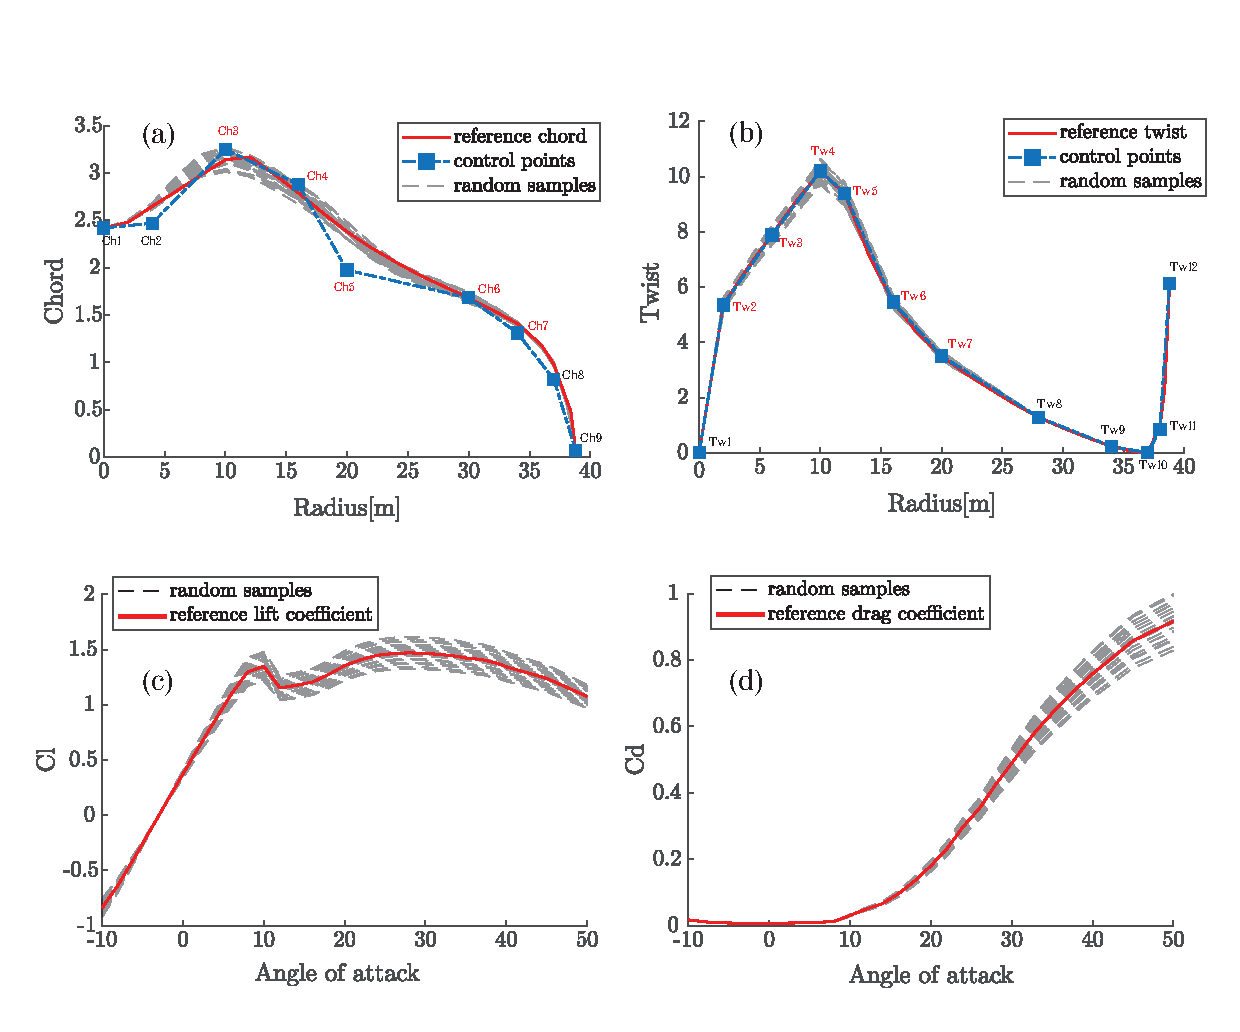
\includegraphics[trim={0.5cm 0cm 0 0cm},clip, scale=0.67]{figure1.pdf}
\caption{Random realization of chord, twist, lift- (Cl2) and drag-polars (Cd2).}
\label{perturbed_samples}
\end{figure}

\subsection{Verification of sensitivity analysis method}
We perform a convergence study for both OLS and LARS in order to determine which method converges fastest with increasing number of uncertain parameters and number of model runs. For this purpose we only include uncertainty in the chord and set the power production as the quantity of interest. The NURBS representation is defined by 9 control points, of which a subset is taken uncertain (see Fig.\ \ref{perturbed_samples}(a)). In Fig.\ \ref{convergence_dim}, we show for both OLS and LARS the convergence behaviour of the total Sobol indices of the power output with increasing number of model evaluations $N$ (runs of the AeroModule), and with increasing number of uncertain inputs $M$ (4, 6 and 8 control points). We see that both methods scale well with increasing dimensions, however, LARS exhibits faster convergence than OLS in high dimensions due to its adaptive nature, and will be the method of choice in the subsequent tests. For both OLS and LARS, we start with a small $N$ and double it with every iteration until converged values of Sobol indices are obtained.
%}  \todo{what is a reasonable choice of $N$, depending on $M$?}

\begin{figure*}[h!]
    \centering
    \begin{subfigure}[t]{0.32\textwidth}
        \centering
        \includegraphics[trim={1cm 0cm 0 0cm}, clip, scale = 0.22]{convergence_chord1_4.eps}{a}
        \caption{$M=4, Ch1-Ch4$}
    \end{subfigure}%
    ~ 
    \begin{subfigure}[t]{0.32\textwidth}
        \centering
        \includegraphics[trim={1cm 0cm 0 0cm},clip, scale=0.22]{convergence_chord1_6.eps}
        \caption{$M=6, Ch1-Ch6$}
    \end{subfigure}
      ~ 
    \begin{subfigure}[t]{0.32\textwidth}
        \centering
        \includegraphics[trim={1cm 0cm 0 0cm},clip, scale=0.22]{convergence_chord1_8.eps}
        \caption{ $M=8, Ch1-Ch8$}
 \end{subfigure}
    \caption{Convergence of OLS and LARS with increasing number of uncertain inputs $M$ (chord control points) and model evaluations $N$.}
\label{convergence_dim}
\end{figure*}

%\FloatBarrier

\subsection{Sensitivity analysis results}
In Fig.~\ref{fig:sensitivity_analysis_power} and \ref{fig:sensitivity_analysis_force}, we show the total order Sobol indices as a measure of the sensitivity of the different geometric and model parameters on the power output and the axial force, respectively, computed using LARS with $M=19$ uncertain parameters chosen from Fig.~\ref{perturbed_samples}. We found that $N=1024$ model evaluations were sufficient to achieve converged indices. In this case, we observe that the uncertainty in model parameters is at least as important as the uncertainty in geometric parameters. Furthermore, within the geometric parameters, the chord distribution shows a significantly higher sensitivity than the twist variables. Lastly, we observe that the axial force is basically only sensitive to the lift coefficient at the outward blade sections, whereas the power is sensitive to both lift and drag coefficients, also at the inward section of the blade. We note that these findings are testcase-specific and might not generalize directly to other turbines or other operational settings. Furthermore, the reported sensitivities depend on the variance that is chosen for the uncertain parameters; in future work we will relate these to values known from design standards.

\begin{figure}[h!]
\centering
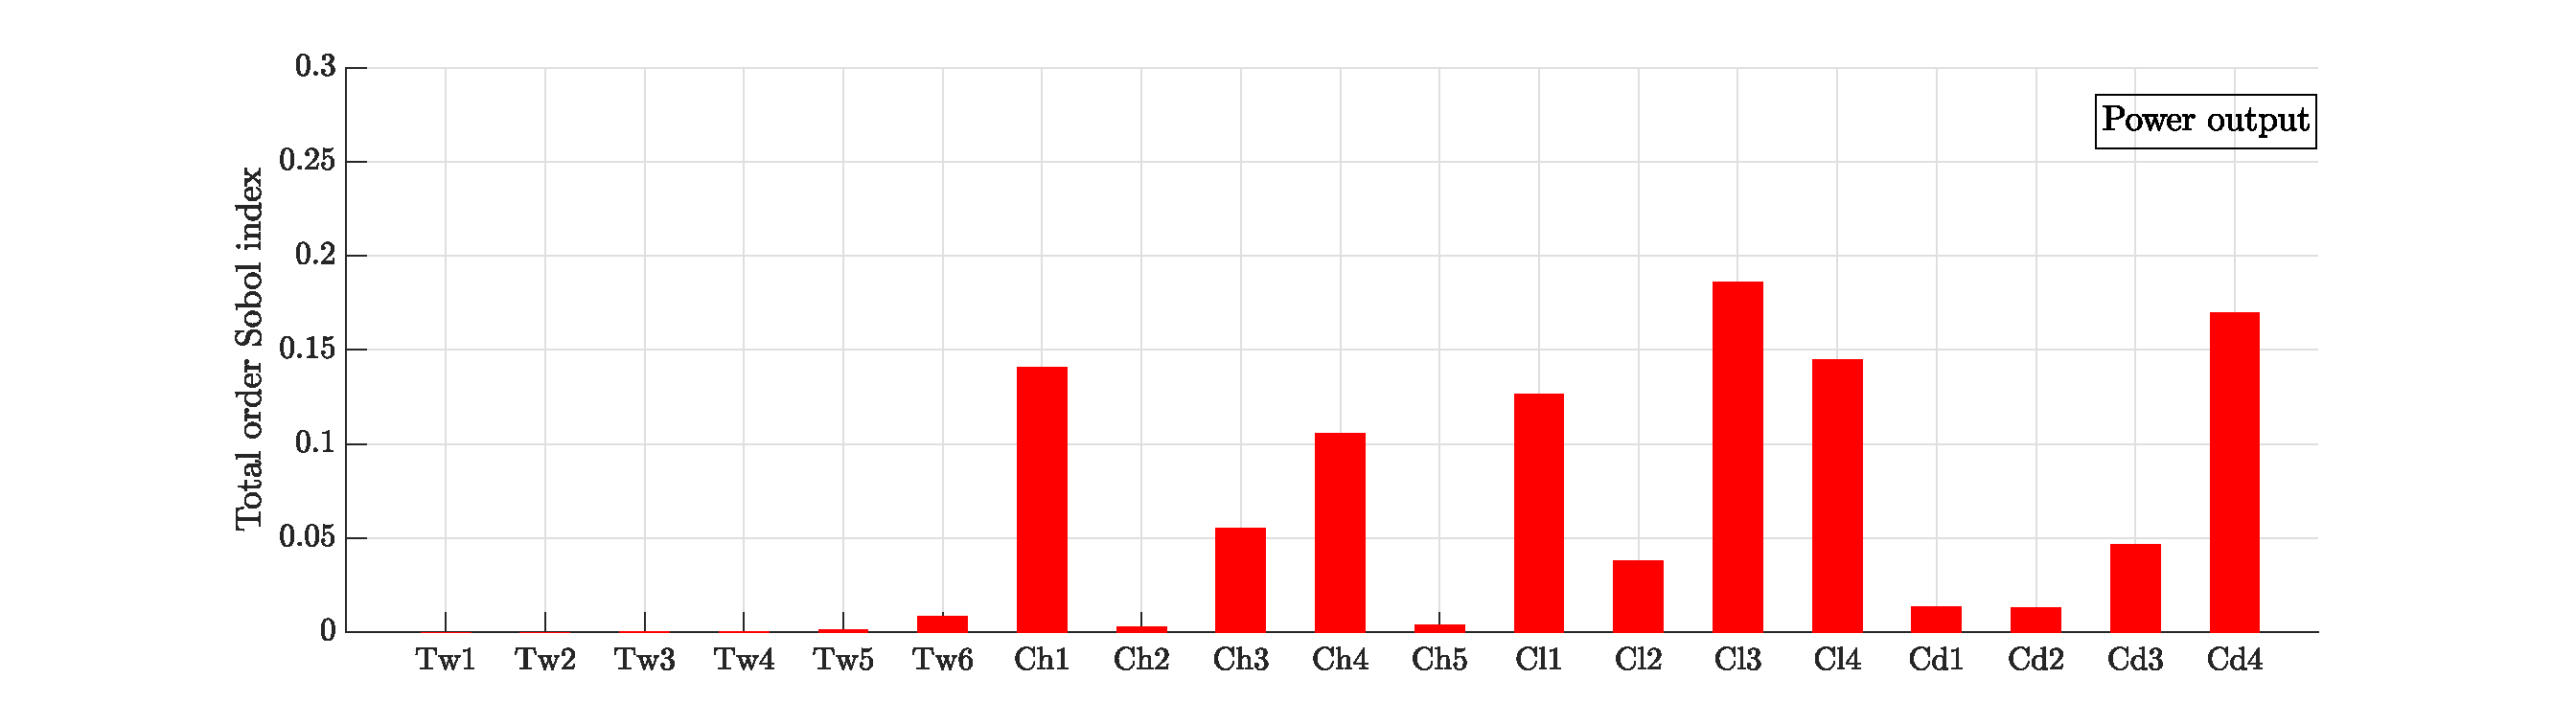
\includegraphics[trim={2cm 0cm 0 0cm},clip, scale=0.4]{SA_Power_chord_twist_Cl_Cd.eps}
\caption{Sensitivity of power output towards geometric and model uncertainties.}
\label{fig:sensitivity_analysis_power}
\end{figure}


\begin{figure}[h!]
\centering
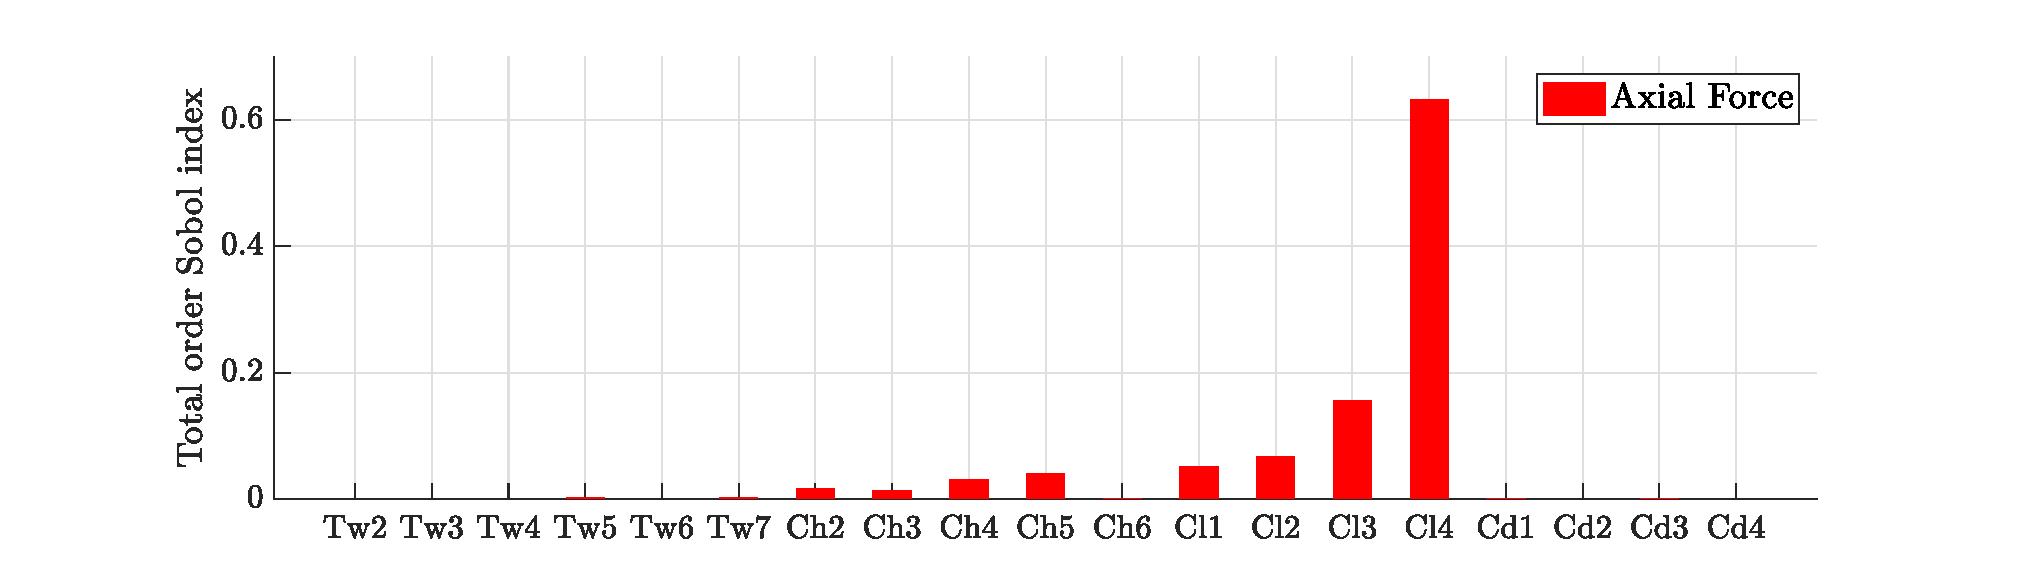
\includegraphics[trim={1cm 0cm 0 0cm},clip, scale=0.5]{SA_axial_force_chord_twist_Cl_Cd.eps}
\caption{Sensitivity of axial force towards geometric and model uncertainties.}
\label{fig:sensitivity_analysis_force}
\end{figure}

%\FloatBarrier

\section{Conclusions}\label{sec:conclusions}
In this paper we have developed a framework for global sensitivity analysis using Sobol indices computed using adaptive sparse polynomial chaos expansions. The framework can be used for high-dimensional global sensitivity analysis of both geometric and model uncertainties in BEM models. As such, the proposed framework is generic and can deal with many types of (parametric) uncertainties, of which a few were investigated in this paper: twist, chord, lift coefficient and drag coefficient. By using NURBS parameterizations of chord, twist, lift and drag as a function of the blade radius, the number of uncertainties was limited but remains considerable (19 uncertain variables). Our approach (adaptive sparse polynomial chaos expansion) is able to efficiently quantify this high-dimensional problem. The results highlight amongst others the importance of the lift coefficient, especially for the axial force prediction. The identified sensitivities will be utilized in future work to develop calibrated BEM models with built-in uncertainty estimates, as part of the \textit{WindTrue} project, and used to better understand the differences between BEM models and measurement data as studied in IEA Task 29. 
